\documentclass[11pt]{article}
\usepackage{graphicx} 
\usepackage{multirow}
\usepackage{enumitem}
\usepackage{amssymb}
\usepackage{amsmath}
\usepackage{amsthm}
\usepackage{xcolor}
\usepackage{array}
\usepackage[simplified]{pgf-umlcd}
\usepackage{minted}
\usepackage{geometry}
  \geometry{
    left = 15mm,
    right = 15mm,
    top = 20mm,
    bottom = 30mm,
  }
\usepackage{fancyhdr}
\renewcommand{\headrulewidth}{0pt}
\pagestyle{fancy}

\setminted{
  fontsize=\small,
  breaklines=true,
  autogobble=true,
  frame=single,
  framesep=3mm
}

\graphicspath{{C:/Users/teoso/Documents/Template Math Depart/}{D:/Hada Touya/Template-Math-Depart/}}

\begin{document}
\pagenumbering{gobble}

\noindent
\begin{minipage}{0.15\textwidth}
  
\includegraphics[width=1.8cm]{ITS.png}
\end{minipage}%
\begin{minipage}{0.7\textwidth}
  \centering
  \textbf{EVALUASI AKHIR SEMESTER - GENAP 2025 / 2026} \\
  \textbf{DEPARTEMEN MATEMATIKA - FSAD ITS} \\
  \vspace{0.3cm}
  \begin{tabular}{l l p{8cm}}
    Mata kuliah / Kode & : & ALGORITMA DAN PEMROGRAMAN 2              \\
    Hari / Tanggal     & : & KAMIS / 18 JUNI 2026                     \\
    Sifat / waktu      & : & TUTUP BUKU / 100 menit                   \\
    Dosen              & : & Dr. Dwi Ratna Sultyaningrum, S.Si., M.T. \\
                       &   & Dr. Budl Setiyono, S.Si., M.T.           \\
                       &   & Alvilda Mustika Rukmil, S.Si., M.Si.     \\
                       &   & Mohammad Iqbal, S.Si., M.Si., Ph.D.
  \end{tabular}
\end{minipage}%
\begin{minipage}{0.15\textwidth}
  \centering
  
\includegraphics[width=1.8cm]{M.png}
\end{minipage}

\vspace{0.5cm}

\noindent \textbf{HARAP DIPERHATIKAN !!!} \\
\textit{Segala jenis pelanggaran (mencontek, kerjasama, dsb) yang dilakukan saat ETS/EAS akan dikenakan sanksi pembatalan mata kuliah pada semester yang sedang berjalan.}

\vspace{0.5cm}

\noindent \textbf{EAS mengukur kemampuan}

\begin{center}
  \begin{tabular}{|c|m{8.6cm}|c|c|c|c|c|c|c|}
    \hline
    \multicolumn{2}{|c|}{\multirow{2}{*}{\textbf{CPMK}} } & \multirow{2}{*}{\textbf{\begin{tabular}{c} BOBOT CPMK \\ (\%) \end{tabular}}}                                                                            & \multicolumn{5}{c|}{\textbf{CPL}}                                                            \\ \cline{4-8}
    \multicolumn{2}{|c|}{ }                               &                                                                                                                                                          & \textbf{4}                        & \textbf{5} & \textbf{7} & \textbf{8} & \textbf{9}        \\ \hline
    1                                                     & Mampu memahami dasar-dasar untuk membangun sebuah algoritma yang benar dan efisien                                                                       &                                   &            &            &            &            &      \\ \hline
    2                                                     & Mampu memahami dan menganalisa algoritma \textit{searching} dan \textit{sorting}                                                                         &                                   &            &            &            &            &      \\ \hline
    3                                                     & Mampu memahami dan mengimplementasikan \textit{Exception Handling}                                                                                       &                                   &            &            &            &            &      \\ \hline
    4                                                     & Mampu memahami dan mengimplementasikan GUI                                                                                                               &                                   &            &            &            &            &      \\ \hline
    5                                                     & Mampu memahami konsep dasar pemrograman berorientasi objek                                                                                               & 25                                &            &            &            & 12.5       & 12.5 \\ \hline
    6                                                     & Mampu menerapkan paradigma pemrograman berorientasi objek dalam mengembangkan suatu program untuk menyelesaikan suatu masalah secara individu maupun tim & 20                                &            &            & 10         &            & 10   \\ \hline
  \end{tabular}
\end{center}

\begin{center}
  \begin{tabular}{|c|c|c|c|c|c|}
    \hline
    \textbf{SOAL}                                   & \textbf{BOBOT SOAL (\%)} & \textbf{CPMK-1} & \textbf{CPMK-2} & \textbf{CPMK-3} & \textbf{CPMK-4} \\ \hline
    \textbf{1}                                      & \textbf{20}              &                 &                 & \textbf{5}      &                 \\ \hline
    \textbf{2}                                      & \textbf{20}              &                 &                 & \textbf{5}      & \textbf{5}      \\ \hline
    \textbf{3}                                      & \textbf{20}              &                 &                 & \textbf{5}      & \textbf{5}      \\ \hline
    \textbf{4}                                      & \textbf{20}              &                 &                 & \textbf{5}      & \textbf{5}      \\ \hline
    \textbf{5}                                      & \textbf{20}              &                 &                 & \textbf{5}      & \textbf{5}      \\ \hline
    \multicolumn{2}{|c|}{\textbf{TOTAL BOBOT CPMK}} &                          &                 & \textbf{25}     & \textbf{20}                       \\ \hline
  \end{tabular}
\end{center}

\begin{enumerate}
  \item \textbf{Enkapsulasi}

        Perhatikan kode yang diberikan:

        \begin{minted}{java}
class Mahasiswa {
    public String nama;
    public double ipk;
}
  \end{minted}

        Kemudian diubah menjadi:

        \begin{minted}{java}
class Mahasiswa {
    private String nama;
    private double ipk;

    public void setNama(String nama) {
        this.nama = nama;
    }

    public String getNama() {
        return nama;
    }
}
  \end{minted}

        \begin{enumerate}[label=\alph*)]
          \item Apa tujuan perubahan tersebut?
          \item Apa keuntungan penggunaan \textit{modifier} \texttt{private}?
          \item Jelaskan manfaat dari teknik enkapsulasi diatas.
        \end{enumerate}

  \item \textbf{Pewarisan (Inheritance)}

        \begin{center}
          \begin{minipage}{0.47\textwidth}
            \begin{minted}{java}
class Barang {
    private String nama;
    private double harga;

    Barang(String nama, double harga) {
        // lengkapi;
    }

    public double getHarga() {
        return harga;
    }
}

class Toko {
    public static void main(String[] args) {
        HargaDiskon produk = new HargaDiskon("Detergen", 15000, 0.2);
        // lengkapi;
    }
}
  \end{minted}
          \end{minipage}
          \hfill
          \begin{minipage}{0.47\textwidth}
            \begin{minted}{java}
class HargaDiskon extends Barang {
    private double diskon;

    HargaDiskon(String nama, double harga, double diskon) {
        // lengkapi;
    }

    public double nettoHarga(int jumlahBarang) {
        // lengkapi;
    }
}
  \end{minted}
          \end{minipage}
        \end{center}

        Lengkapi program di atas pada:
        \begin{enumerate}[label=\alph*)]
          \item Constructor pada kelas \texttt{Barang} dan kelas \texttt{HargaDiskon}
          \item Method \texttt{nettoHarga} dimana jumlah barang $\geq 8$ maka mendapatkan diskon.
          \item Kelas \texttt{Toko} untuk menampilkan output: Harga Netto = 12000 dengan memasukkan jumlah barang 10.
        \end{enumerate}

  \item \textbf{Polimorfisme (Polymorphism)}

        Perhatikan listing program dibawah, jawab pertanyaan berikut :

        \begin{minted}{java}
package EAS2026;
public class SoalPolymorphisme {
    public static void main(String[] args) {
        Kendaraan s = new Sepeda();      // baris A
        s.info();
        s.jalan();
        Kendaraan k = new Mobil();       // baris B
        k.jalan();
        //k.klakson();                   // baris C (di-comment)
    }
}

class Kendaraan {
    void info() { System.out.println("Kendaraan umum"); }
    void jalan() { System.out.println("Tancap gas ...."); }
}

class Mobil extends Kendaraan {
    @Override
    void info() { System.out.println("Ini Mobil"); }
    void klakson() { System.out.println("Tin tin!"); }
}

class Sepeda extends Kendaraan {
    @Override
    void info() { System.out.println("Ini Sepeda"); }
    void jalan() { System.out.println("Putar gas ...."); }
}
  \end{minted}

        \begin{enumerate}[label=\alph*)]
          \item Apa yang terjadi pada baris A dan baris B? Sebutkan istilah teknisnya!
          \item Mengapa baris C akan error jika di-\textit{uncomment}? Jelaskan!
          \item Tuliskan output program diatas.
        \end{enumerate}

  \item \textbf{Abstract dan Interface}

        Perhatikan class diagram berikut :

        \begin{center}
          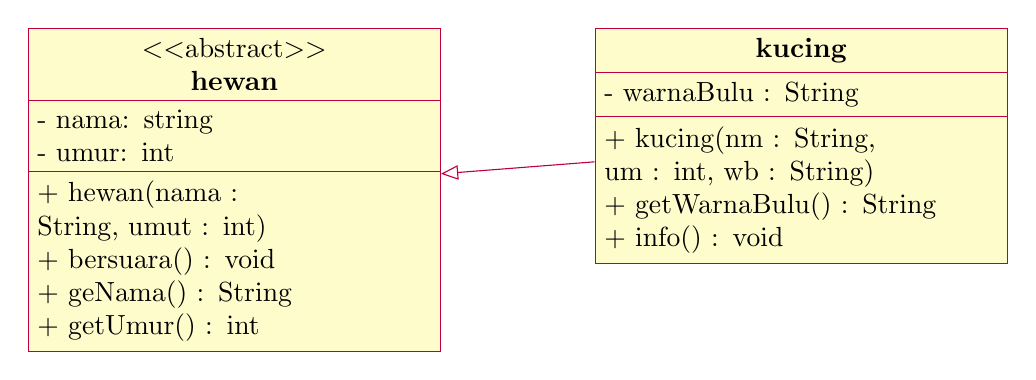
\begin{tikzpicture}
            \begin{abstractclass}{hewan}{0,0}
              \attribute{- nama: string}
              \attribute{- umur: int}
              \operation{+ hewan(nama : String, umut : int)}
              \operation{+ bersuara() : void}
              \operation{+ geNama() : String}
              \operation{+ getUmur() : int}
            \end{abstractclass}

            \begin{class}{kucing}{7.2,0}
              \attribute{- warnaBulu : String}
              \operation{+ kucing(nm : String, um : int, wb : String)}
              \operation{+ getWarnaBulu() : String}
              \operation{+ info() : void}
              \inherit{hewan}
            \end{class}
          \end{tikzpicture}
        \end{center}

        \begin{enumerate}[label=\alph*)]
          \item Implementasikan class diagram tersebut\\
                Keterangan :
                \begin{itemize}
                  \item \textbf{bersuara} akan mencetak ``meong''
                  \item \textbf{info} akan mencetak nama, umur, warna bulu dan bersuara
                \end{itemize}
          \item Buat sebuah obyek, lalu dengan menggunakan obyek tersebut jalankan method \textbf{info}.
        \end{enumerate}

  \item \textbf{Enkapsulasi}

        Desain Kelas untuk sistem perpustakaan. Perhatikan skenario yang diberikan.
        \begin{center}
          \fbox{%
            \begin{minipage}{0.92\textwidth}
              \textbf{Skenario}\\[1mm]
              Perpustakaan kampus ingin membuat sistem peminjaman buku. Setiap buku memiliki kode ISBN (unik, tidak berubah), judul, nama pengarang, dan status ketersediaan (tersedia atau dipinjam). Status hanya boleh berubah melalui dua aksi resmi: pinjam dan kembalikan. Ketika buku dipinjam, sistem harus memastikan buku dalam kondisi tersedia. Ketika dikembalikan, buku harus dalam kondisi sedang dipinjam.
            \end{minipage}
          }
        \end{center}

        \begin{enumerate}[label=\alph*)]
          \item Rancang daftar atribut kelas Buku beserta akses modifier yang tepat untuk masing-masing. Jelaskan pilihan Anda!
          \item Mengapa atribut status ketersediaan tidak boleh memiliki setter public biasa seperti \texttt{setStatus(Boolean status)}? Apa risikonya jika dibuat?
          \item Jika kelas lain ingin mengecek apakah buku tersedia sebelum meminjam, mekanisme apa yang sebaiknya disediakan kelas Buku?
        \end{enumerate}
\end{enumerate}

\newpage
\begin{center}
  \textbf{SOLUSI}
\end{center}
\begin{enumerate}
  \item
        \begin{enumerate}[label=\alph*)]
          \item Tujuan perubahan adalah membatasi akses langsung ke data objek dan memaksa akses melalui method yang terkontrol. Dengan begitu data lebih aman dan aturan validasi bisa diterapkan.

          \item Keuntungan \texttt{private} adalah atribut tidak bisa diubah sembarangan dari luar kelas, sehingga integritas data terjaga dan implementasi internal bisa diubah tanpa memengaruhi pemakai kelas.

          \item Manfaat enkapsulasi adalah menyembunyikan detail implementasi, menjaga konsistensi objek, memudahkan perawatan kode, dan membuat kelas lebih aman untuk digunakan.
        \end{enumerate}

  \item
        \begin{enumerate}[label=\alph*)]
          \item Constructor pada kelas \texttt{Barang} dan kelas \texttt{HargaDiskon}:
                \begin{minted}{java}
    Barang(String nama, double harga) {
        this.nama = nama;
        this.harga = harga;
    }

    HargaDiskon(String nama, double harga, double diskon) {
        super(nama, harga);
        this.diskon = diskon;
    }
                \end{minted}

          \item Method \texttt{nettoHarga}:
                \begin{minted}{java}
    public double nettoHarga(int jumlahBarang) {
        if (jumlahBarang >= 8) {
            return getHarga() - (getHarga() * diskon);
        }
        return getHarga();
    }
                \end{minted}

          \item Kelas \texttt{Toko}:
                \begin{minted}{java}
class Toko {
    public static void main(String[] args) {
        HargaDiskon produk = new HargaDiskon("Detergen", 15000, 0.2);
        System.out.println("Harga Netto = " + produk.nettoHarga(10));
    }
}
                \end{minted}
        \end{enumerate}

  \item
        \begin{enumerate}[label=\alph*)]
          \item Baris A dan B melakukan \textit{upcasting}, yaitu objek turunan disimpan ke referensi kelas induk. Saat method di-override, pemanggilan method mengikuti objek sebenarnya pada runtime, sehingga terjadi \textit{dynamic dispatch}.

          \item Baris C error jika di-uncomment karena variabel \texttt{k} bertipe \texttt{Kendaraan}, sedangkan \texttt{Kendaraan} tidak memiliki method \texttt{klakson()}. Method tersebut hanya ada di \texttt{Mobil}, jadi tidak bisa dipanggil lewat referensi induk.

          \item Output program:
                \begin{verbatim}
Ini Sepeda
Putar gas ....
Tancap gas ....
                \end{verbatim}
        \end{enumerate}

  \item
        \begin{enumerate}[label=\alph*)]
          \item Implementasi class \texttt{Hewan} dan \texttt{Kucing}:
                \begin{minted}{java}
abstract class Hewan {
    private String nama;
    private int umur;

    Hewan(String nama, int umur) {
        this.nama = nama;
        this.umur = umur;
    }

    public String getNama() {
        return nama;
    }

    public int getUmur() {
        return umur;
    }

    public abstract void bersuara();
}

class Kucing extends Hewan {
    private String warnaBulu;

    Kucing(String nama, int umur, String warnaBulu) {
        super(nama, umur);
        this.warnaBulu = warnaBulu;
    }

    public String getWarnaBulu() {
        return warnaBulu;
    }

    @Override
    public void bersuara() {
        System.out.println("meong");
    }

    public void info() {
        System.out.println("Nama: " + getNama());
        System.out.println("Umur: " + getUmur());
        System.out.println("Warna bulu: " + getWarnaBulu());
        bersuara();
    }
}
                \end{minted}

          \item Membuat objek dan memanggil method \texttt{info}:
                \begin{minted}{java}
class DemoKucing {
    public static void main(String[] args) {
        Kucing kucing = new Kucing("Mimi", 2, "Putih");
        kucing.info();
    }
}
                \end{minted}
        \end{enumerate}

  \item
        \begin{enumerate}[label=\alph*)]
          \item Atribut kelas \texttt{Buku} yang dirancang:
                \begin{itemize}
                  \item \texttt{private final String isbn}: \textit{Modifier} \texttt{private} untuk menyembunyikan data dari luar kelas. Tambahan \texttt{final} digunakan karena kode ISBN bersifat unik untuk setiap buku dan tidak boleh berubah setelah objek buku dibuat.
                  \item \texttt{private String judul}: \textit{Modifier} \texttt{private} untuk menjaga enkapsulasi, sehingga judul hanya bisa diakses/diubah (jika diperlukan) melalui \textit{method} yang disediakan.
                  \item \texttt{private String pengarang}: Sama seperti judul, \texttt{private} digunakan untuk melindungi data agar tidak diakses langsung dari luar.
                  \item \texttt{private boolean tersedia}: \textit{Modifier} \texttt{private} sangat krusial di sini agar status peminjaman tidak bisa diubah langsung dari luar. Perubahan status hanya diizinkan melalui \textit{method} resmi yaitu \texttt{pinjam()} dan \texttt{kembalikan()}.
                \end{itemize}

          \item \texttt{status} tidak boleh punya \textit{setter public} biasa (seperti \texttt{setStatus(boolean status)}) karena hal tersebut akan merusak logika bisnis peminjaman. Risiko jika dibuat: kelas lain bisa sembarangan mengubah status buku yang sedang dipinjam menjadi tersedia (atau sebaliknya) tanpa melalui proses validasi (misal mengecek apakah buku benar-benar sedang dipinjam sebelum dikembalikan).

          \item Mekanisme yang sebaiknya disediakan adalah \textit{method getter/accessor} yang mengembalikan nilai boolean, contohnya \texttt{isTersedia()} atau \texttt{getTersedia()}. Dengan begitu, kelas lain bisa mengecek kondisi buku tanpa memiliki akses untuk mengubah nilainya.
        \end{enumerate}
\end{enumerate}

\end{document}
